\documentclass[tikz,border=2pt]{standalone}
\usepackage{amsmath,amssymb}
\usepackage{tikz}
\usetikzlibrary{arrows.meta,positioning}

\begin{document}
% Project network with activities on the edges (durations): the project length is the
% LONGEST path from S to T, here 9 along S-2-3-T (and S-1-3-T), the critical path(s).
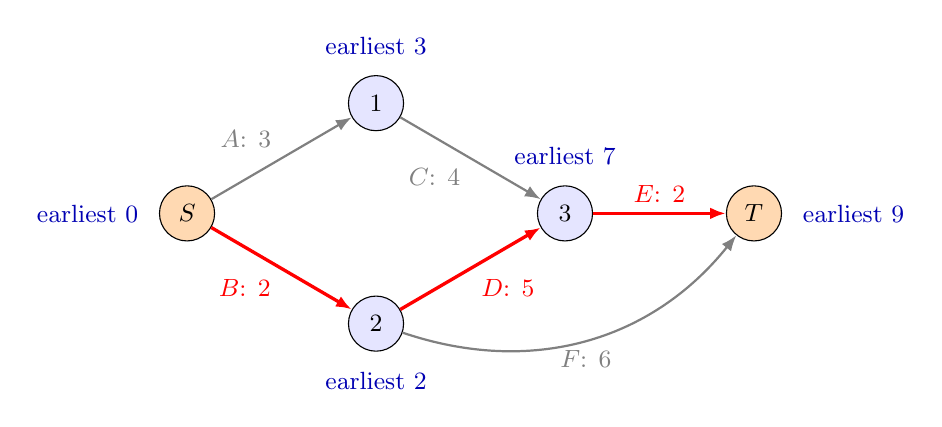
\begin{tikzpicture}[every node/.style={font=\small}, >={Latex[length=2mm]}, v/.style={draw, circle, fill=blue!10, minimum size=7mm, inner sep=0pt}]
	\node[v, fill=orange!30] (S) at (0,0) {$S$};
	\node[v] (n1) at (2.4,1.4) {$1$};
	\node[v] (n2) at (2.4,-1.4) {$2$};
	\node[v] (n3) at (4.8,0) {$3$};
	\node[v, fill=orange!30] (T) at (7.2,0) {$T$};
	\draw[->, thick, gray] (S) -- (n1) node[midway, above left, font=\small] {$A$: $3$};
	\draw[->, very thick, red] (S) -- (n2) node[midway, below left, font=\small] {$B$: $2$};
	\draw[->, thick, gray] (n1) -- (n3) node[midway, below left, font=\small] {$C$: $4$};
	\draw[->, very thick, red] (n2) -- (n3) node[midway, below right, font=\small] {$D$: $5$};
	\draw[->, very thick, red] (n3) -- (T) node[midway, above, font=\small] {$E$: $2$};
	\draw[->, thick, gray] (n2) to[bend right=35] node[midway, below, font=\small] {$F$: $6$} (T);
	\foreach \n/\e/\p in {S/0/{left}, n1/3/{above}, n2/2/{below}, n3/7/{above}, T/9/{right}} {\node[blue!70!black, font=\small, \p=4pt of \n] {earliest $\e$};}
	\end{tikzpicture}
\end{document}
